\hypertarget{stm32f4xx__hal__tim_8c}{}\section{Dokumentacja pliku S\+T\+M/\+W\+D\+S\+\_\+\+Kosc\+\_\+\+Linux/\+Drivers/\+S\+T\+M32\+F4xx\+\_\+\+H\+A\+L\+\_\+\+Driver/\+Src/stm32f4xx\+\_\+hal\+\_\+tim.c}
\label{stm32f4xx__hal__tim_8c}\index{S\+T\+M/\+W\+D\+S\+\_\+\+Kosc\+\_\+\+Linux/\+Drivers/\+S\+T\+M32\+F4xx\+\_\+\+H\+A\+L\+\_\+\+Driver/\+Src/stm32f4xx\+\_\+hal\+\_\+tim.\+c@{S\+T\+M/\+W\+D\+S\+\_\+\+Kosc\+\_\+\+Linux/\+Drivers/\+S\+T\+M32\+F4xx\+\_\+\+H\+A\+L\+\_\+\+Driver/\+Src/stm32f4xx\+\_\+hal\+\_\+tim.\+c}}


T\+IM H\+AL module driver. This file provides firmware functions to manage the following functionalities of the Timer (T\+IM) peripheral\+:  


{\ttfamily \#include \char`\"{}stm32f4xx\+\_\+hal.\+h\char`\"{}}\newline
Wykres zależności załączania dla stm32f4xx\+\_\+hal\+\_\+tim.\+c\+:\nopagebreak
\begin{figure}[H]
\begin{center}
\leavevmode
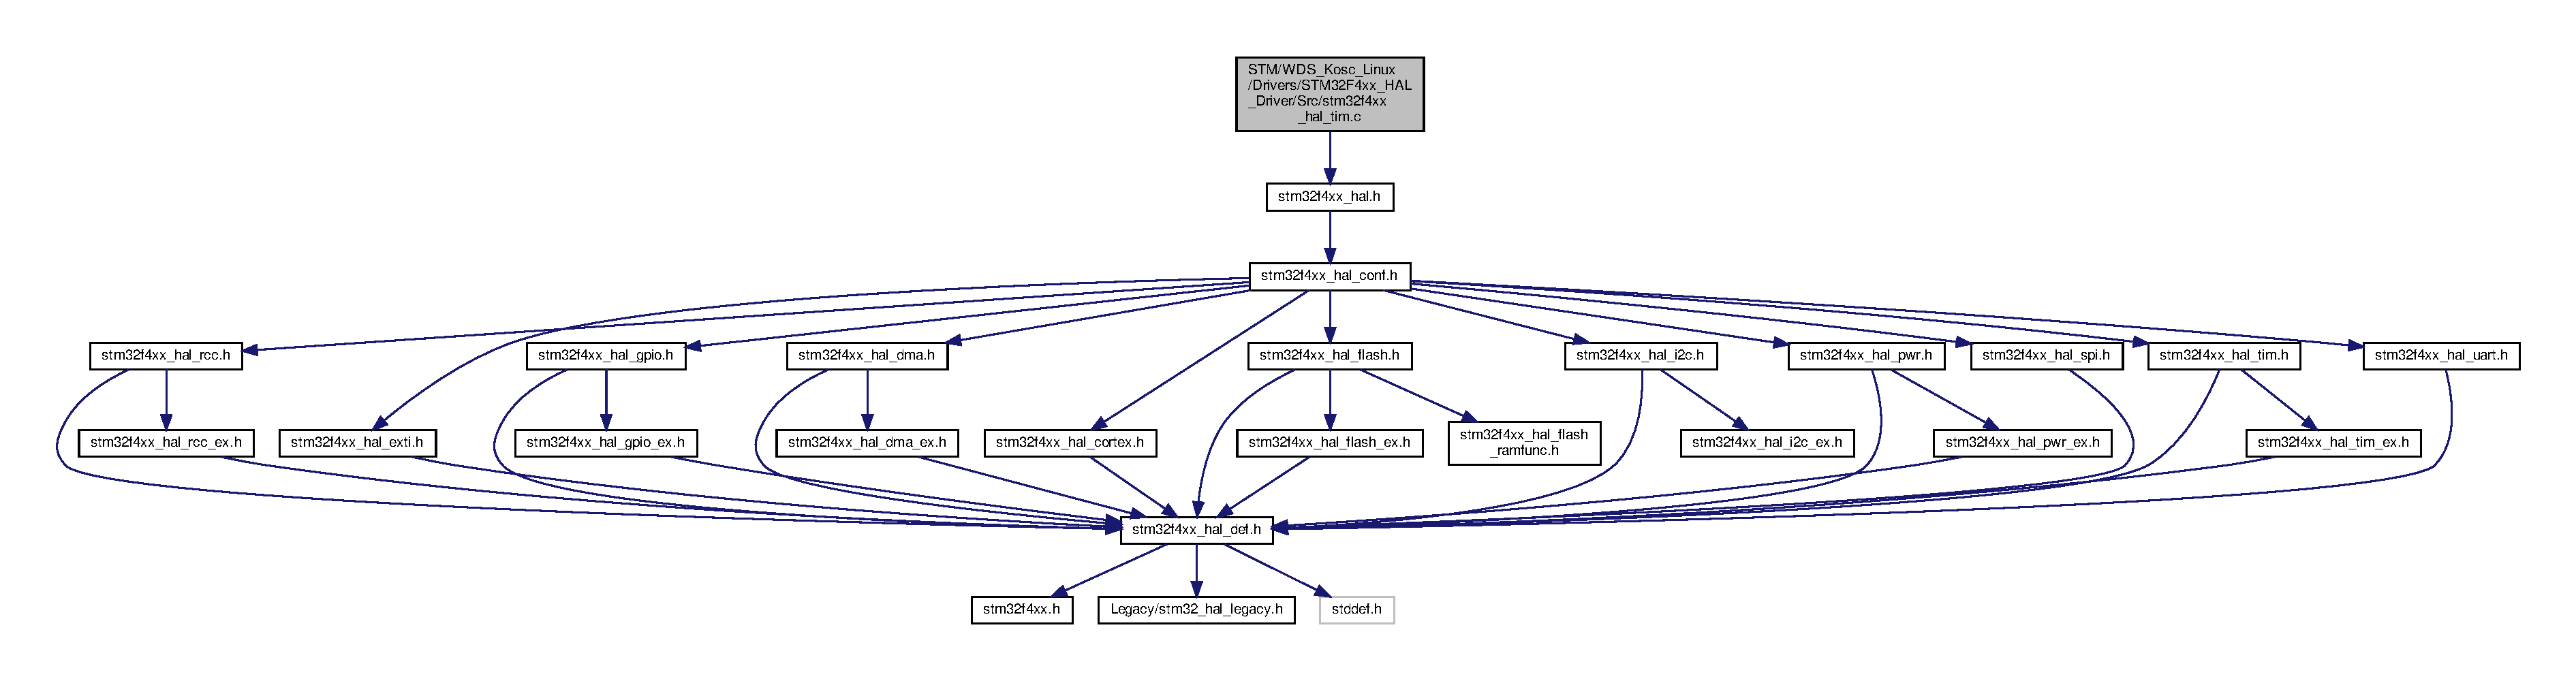
\includegraphics[width=350pt]{stm32f4xx__hal__tim_8c__incl}
\end{center}
\end{figure}


\subsection{Opis szczegółowy}
T\+IM H\+AL module driver. This file provides firmware functions to manage the following functionalities of the Timer (T\+IM) peripheral\+: 

\begin{DoxyAuthor}{Autor}
M\+CD Application Team
\begin{DoxyItemize}
\item T\+IM Time Base Initialization
\item T\+IM Time Base Start
\item T\+IM Time Base Start Interruption
\item T\+IM Time Base Start D\+MA
\item T\+IM Output Compare/\+P\+WM Initialization
\item T\+IM Output Compare/\+P\+WM Channel Configuration
\item T\+IM Output Compare/\+P\+WM Start
\item T\+IM Output Compare/\+P\+WM Start Interruption
\item T\+IM Output Compare/\+P\+WM Start D\+MA
\item T\+IM Input Capture Initialization
\item T\+IM Input Capture Channel Configuration
\item T\+IM Input Capture Start
\item T\+IM Input Capture Start Interruption
\item T\+IM Input Capture Start D\+MA
\item T\+IM One Pulse Initialization
\item T\+IM One Pulse Channel Configuration
\item T\+IM One Pulse Start
\item T\+IM Encoder Interface Initialization
\item T\+IM Encoder Interface Start
\item T\+IM Encoder Interface Start Interruption
\item T\+IM Encoder Interface Start D\+MA
\item Commutation Event configuration with Interruption and D\+MA
\item T\+IM O\+C\+Ref clear configuration
\item T\+IM External Clock configuration \begin{DoxyVerb}  ==============================================================================
                      ##### TIMER Generic features #####
  ==============================================================================
  [..] The Timer features include:
       (#) 16-bit up, down, up/down auto-reload counter.
       (#) 16-bit programmable prescaler allowing dividing (also on the fly) the
           counter clock frequency either by any factor between 1 and 65536.
       (#) Up to 4 independent channels for:
           (++) Input Capture
           (++) Output Compare
           (++) PWM generation (Edge and Center-aligned Mode)
           (++) One-pulse mode output
       (#) Synchronization circuit to control the timer with external signals and to interconnect
            several timers together.
       (#) Supports incremental encoder for positioning purposes

            ##### How to use this driver #####
  ==============================================================================
    [..]
     (#) Initialize the TIM low level resources by implementing the following functions
         depending on the selected feature:
           (++) Time Base : HAL_TIM_Base_MspInit()
           (++) Input Capture : HAL_TIM_IC_MspInit()
           (++) Output Compare : HAL_TIM_OC_MspInit()
           (++) PWM generation : HAL_TIM_PWM_MspInit()
           (++) One-pulse mode output : HAL_TIM_OnePulse_MspInit()
           (++) Encoder mode output : HAL_TIM_Encoder_MspInit()

     (#) Initialize the TIM low level resources :
        (##) Enable the TIM interface clock using __HAL_RCC_TIMx_CLK_ENABLE();
        (##) TIM pins configuration
            (+++) Enable the clock for the TIM GPIOs using the following function:
             __HAL_RCC_GPIOx_CLK_ENABLE();
            (+++) Configure these TIM pins in Alternate function mode using HAL_GPIO_Init();

     (#) The external Clock can be configured, if needed (the default clock is the
         internal clock from the APBx), using the following function:
         HAL_TIM_ConfigClockSource, the clock configuration should be done before
         any start function.

     (#) Configure the TIM in the desired functioning mode using one of the
       Initialization function of this driver:
       (++) HAL_TIM_Base_Init: to use the Timer to generate a simple time base
       (++) HAL_TIM_OC_Init and HAL_TIM_OC_ConfigChannel: to use the Timer to generate an
            Output Compare signal.
       (++) HAL_TIM_PWM_Init and HAL_TIM_PWM_ConfigChannel: to use the Timer to generate a
            PWM signal.
       (++) HAL_TIM_IC_Init and HAL_TIM_IC_ConfigChannel: to use the Timer to measure an
            external signal.
       (++) HAL_TIM_OnePulse_Init and HAL_TIM_OnePulse_ConfigChannel: to use the Timer
            in One Pulse Mode.
       (++) HAL_TIM_Encoder_Init: to use the Timer Encoder Interface.

     (#) Activate the TIM peripheral using one of the start functions depending from the feature used:
           (++) Time Base : HAL_TIM_Base_Start(), HAL_TIM_Base_Start_DMA(), HAL_TIM_Base_Start_IT()
           (++) Input Capture :  HAL_TIM_IC_Start(), HAL_TIM_IC_Start_DMA(), HAL_TIM_IC_Start_IT()
           (++) Output Compare : HAL_TIM_OC_Start(), HAL_TIM_OC_Start_DMA(), HAL_TIM_OC_Start_IT()
           (++) PWM generation : HAL_TIM_PWM_Start(), HAL_TIM_PWM_Start_DMA(), HAL_TIM_PWM_Start_IT()
           (++) One-pulse mode output : HAL_TIM_OnePulse_Start(), HAL_TIM_OnePulse_Start_IT()
           (++) Encoder mode output : HAL_TIM_Encoder_Start(), HAL_TIM_Encoder_Start_DMA(), HAL_TIM_Encoder_Start_IT().

     (#) The DMA Burst is managed with the two following functions:
         HAL_TIM_DMABurst_WriteStart()
         HAL_TIM_DMABurst_ReadStart()

    *** Callback registration ***
  =============================================

  [..]
  The compilation define  USE_HAL_TIM_REGISTER_CALLBACKS when set to 1
  allows the user to configure dynamically the driver callbacks.

  [..]
  Use Function @ref HAL_TIM_RegisterCallback() to register a callback.
  @ref HAL_TIM_RegisterCallback() takes as parameters the HAL peripheral handle,
  the Callback ID and a pointer to the user callback function.

  [..]
  Use function @ref HAL_TIM_UnRegisterCallback() to reset a callback to the default
  weak function.
  @ref HAL_TIM_UnRegisterCallback takes as parameters the HAL peripheral handle,
  and the Callback ID.

  [..]
  These functions allow to register/unregister following callbacks:
    (+) Base_MspInitCallback              : TIM Base Msp Init Callback.
    (+) Base_MspDeInitCallback            : TIM Base Msp DeInit Callback.
    (+) IC_MspInitCallback                : TIM IC Msp Init Callback.
    (+) IC_MspDeInitCallback              : TIM IC Msp DeInit Callback.
    (+) OC_MspInitCallback                : TIM OC Msp Init Callback.
    (+) OC_MspDeInitCallback              : TIM OC Msp DeInit Callback.
    (+) PWM_MspInitCallback               : TIM PWM Msp Init Callback.
    (+) PWM_MspDeInitCallback             : TIM PWM Msp DeInit Callback.
    (+) OnePulse_MspInitCallback          : TIM One Pulse Msp Init Callback.
    (+) OnePulse_MspDeInitCallback        : TIM One Pulse Msp DeInit Callback.
    (+) Encoder_MspInitCallback           : TIM Encoder Msp Init Callback.
    (+) Encoder_MspDeInitCallback         : TIM Encoder Msp DeInit Callback.
    (+) HallSensor_MspInitCallback        : TIM Hall Sensor Msp Init Callback.
    (+) HallSensor_MspDeInitCallback      : TIM Hall Sensor Msp DeInit Callback.
    (+) PeriodElapsedCallback             : TIM Period Elapsed Callback.
    (+) PeriodElapsedHalfCpltCallback     : TIM Period Elapsed half complete Callback.
    (+) TriggerCallback                   : TIM Trigger Callback.
    (+) TriggerHalfCpltCallback           : TIM Trigger half complete Callback.
    (+) IC_CaptureCallback                : TIM Input Capture Callback.
    (+) IC_CaptureHalfCpltCallback        : TIM Input Capture half complete Callback.
    (+) OC_DelayElapsedCallback           : TIM Output Compare Delay Elapsed Callback.
    (+) PWM_PulseFinishedCallback         : TIM PWM Pulse Finished Callback.
    (+) PWM_PulseFinishedHalfCpltCallback : TIM PWM Pulse Finished half complete Callback.
    (+) ErrorCallback                     : TIM Error Callback.
    (+) CommutationCallback               : TIM Commutation Callback.
    (+) CommutationHalfCpltCallback       : TIM Commutation half complete Callback.
    (+) BreakCallback                     : TIM Break Callback.

  [..]
By default, after the Init and when the state is HAL_TIM_STATE_RESET
all interrupt callbacks are set to the corresponding weak functions:
  examples @ref HAL_TIM_TriggerCallback(), @ref HAL_TIM_ErrorCallback().

  [..]
  Exception done for MspInit and MspDeInit functions that are reset to the legacy weak
  functionalities in the Init / DeInit only when these callbacks are null
  (not registered beforehand). If not, MspInit or MspDeInit are not null, the Init / DeInit
    keep and use the user MspInit / MspDeInit callbacks(registered beforehand)

  [..]
    Callbacks can be registered / unregistered in HAL_TIM_STATE_READY state only.
    Exception done MspInit / MspDeInit that can be registered / unregistered
    in HAL_TIM_STATE_READY or HAL_TIM_STATE_RESET state,
    thus registered(user) MspInit / DeInit callbacks can be used during the Init / DeInit.
  In that case first register the MspInit/MspDeInit user callbacks
      using @ref HAL_TIM_RegisterCallback() before calling DeInit or Init function.

  [..]
      When The compilation define USE_HAL_TIM_REGISTER_CALLBACKS is set to 0 or
      not defined, the callback registration feature is not available and all callbacks
      are set to the corresponding weak functions.\end{DoxyVerb}

\end{DoxyItemize}
\end{DoxyAuthor}
\begin{DoxyAttention}{Uwaga}

\end{DoxyAttention}
\subsubsection*{\begin{center}\copyright{} Copyright (c) 2016 S\+T\+Microelectronics. All rights reserved.\end{center} }

This software component is licensed by ST under B\+SD 3-\/\+Clause license, the \char`\"{}\+License\char`\"{}; You may not use this file except in compliance with the License. You may obtain a copy of the License at\+: opensource.\+org/licenses/\+B\+S\+D-\/3-\/\+Clause 